\cotefile{64}
\scanpage{78}
\mspage{3}
% archive foliation: 77

où $Q_0$ est un carré donné une fois pour toutes (\unsure{$k$} étant fixé\deleted{\unsure{?}}, disons, quand même), avec comme seule donnée un iso
\[
(16)\qquad \underline{\omega}_{Q_0}\deleted{\unsure{Q_0}}\simeq\mu_4^* \qquad\text{i.e. d'un \unsure{élément} de }\mu_4^*\wedge\underline{\omega}_{Q_0}
\]
i.e. un isom.
\[
(17)\qquad \mu_4^{\deleted{\unsure{*}}}\simeq\operatorname{Aut}^{+}(Q_0).
\]

Pour des raisons qui apparaîtront par la suite, le choix le plus opportun est de prendre pour $Q_0$ le carré \deleted{\unsure{ainsi} satisfaisant}\inserted{donné} (17), avec un côté fixé, dont \deleted{les extrémités}\inserted{\unsure{l'ens|l'une} des \unsure{2} extrémités} $s,s'$ \deleted{\unsure{est}} dans une corr. biunivoque avec l'ens. $\mu_4^*=\{i,i'\}$ des racines carrées de $-1$, par la condition que
\[
\deleted{\unsure{s'=i_s s}}
\]
\figure{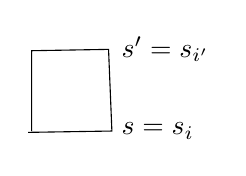
\begin{tikzpicture}[scale=.85]
\draw (0,0)--(0,1.2)--(1.15,1.22)--(1.2,0)--(-.05,-.02);
\node[anchor=west] at (1.2,1.22) {$s'=s_{i'}$};
\node[anchor=west] at (1.2,0) {$s=s_i$};
\end{tikzpicture}}
\[
(18)\qquad \deleted{\unsure{s_{i'}=}}s_{i'}=i\,s_i\qquad\text{d'où}\qquad s_i=i'\,s_{i'}
\]
puisque $i'=i^{-1}=-i$. Ainsi, $T_0$ peut s'interpréter comme \unsure{muni} de la structure \deleted{\unsure{par}}\inserted{suivante, \unsure{qui le caractérise} :} $T_0\otimes\underline{U}_{\unsure{t|4}}(-1)$ est muni d'une paire de bases, \deleted{\unsure{reliées entre}}\inserted{en corr. $1$-$1$} avec $\mu_4^*$, satisfaisant les mêmes relations (18); où maintenant le produit $i\,s_i$ est au sens de la structure vectorielle de $T_0\otimes\underline{U}_{\unsure{t|4}}(-1)$. \deleted{\unsure{Si}}

Ici on aura un iso. canonique
\[
(19)\qquad D_{Q_0}\simeq\mu_4^*
\]
et par suite la donnée (16) équivaut à la donnée d'un iso
